%%%%%%%%%%%%%%%%%%%%%%%%%%%%%%%%%%%%%%%%%%%%%%%%%%%%%%%%%%%%%%%%%%%%%%%%
%                                                                      %
%     File: Thesis_Introduction.tex                                    %
%     Tex Master: Thesis.tex                                           %
%                                                                      %
%     Author: Andre C. Marta                                           %
%     Last modified :  4 Mar 2024                                      %
%                                                                      %
%%%%%%%%%%%%%%%%%%%%%%%%%%%%%%%%%%%%%%%%%%%%%%%%%%%%%%%%%%%%%%%%%%%%%%%%

\chapter{Introduction}
\label{chapter:introduction}


%%%%%%%%%%%%%%%%%%%%%%%%%%%%%%%%%%%%%%%%%%%%%%%%%%%%%%%%%%%%%%%%%%%%%%%%
\section{Motivation}
\label{section:motivation}
Saving lives at sea, protecting marine ecosystems, and securing maritime infrastructure all rely on one essential capability: understanding what is happening, where, and when. In vast and dynamic maritime environments, this requires maintaining reliable, high-resolution situational awareness over long periods. The \gls{emsa} recognises this challenge and highlights the need for continuous monitoring and locally persistent operations to enable effective maritime surveillance and response~\cite{europeanmaritimesafetyagencyEMSAOutlook2025_v302025}.

Different maritime assets meet this challenge in complementary ways. 
Surface vessels give a physical presence at sea, with long endurance and large payload capacity~\cite{introduction_motivation_vessel_sensors,introduction_motivation_vessel_tasks}. 
However, their range is limited by line of sight, and operations are expensive~\cite{introduction_motivation_vessel_limitations}. 
Aerial platforms, such as manned aircraft and \glspl{uav}, allow fast deployment and elevated sensing~\cite{introduction_motivation_aerial_surveillance}. 
Yet, aircraft are costly, and \glspl{uav} suffer from low endurance and unreliable communication~\cite{introduction_motivation_uavs_limitations}.

Together, these assets form a connected system rather than separate solutions. 
Each one compensates for what the other lacks. 
\glspl{usv} provides long-term presence at sea at much lower cost than crewed vessels, allowing wide and affordable patrols. 
\glspl{uav} extend this reach by sensing beyond the horizon from the air. 
Working as a team, they maintain continuous and local maritime awareness. 
This motivates the study of coordinated \gls{usv}--\gls{uav} systems, where cooperation creates mission capabilities that neither platform can achieve alone in complex and changing environments.


A natural way to strengthen this cooperation is to add a physical tether between both platforms. 
The tether provides continuous power and reliable communication between the \gls{usv} and \gls{uav}~\cite{introduction_motivation_tethered_drones}. 
By placing the energy supply and communication systems on the \gls{usv}, it overcomes two main limits of maritime \glspl{uav}: short endurance and weak long-range communication.

Figure~\ref{fig:tether_scheme} illustrates the configuration of the tethered \gls{usv}--\gls{uav} system considered in this work.

\begin{figure}[H]
    \centering
    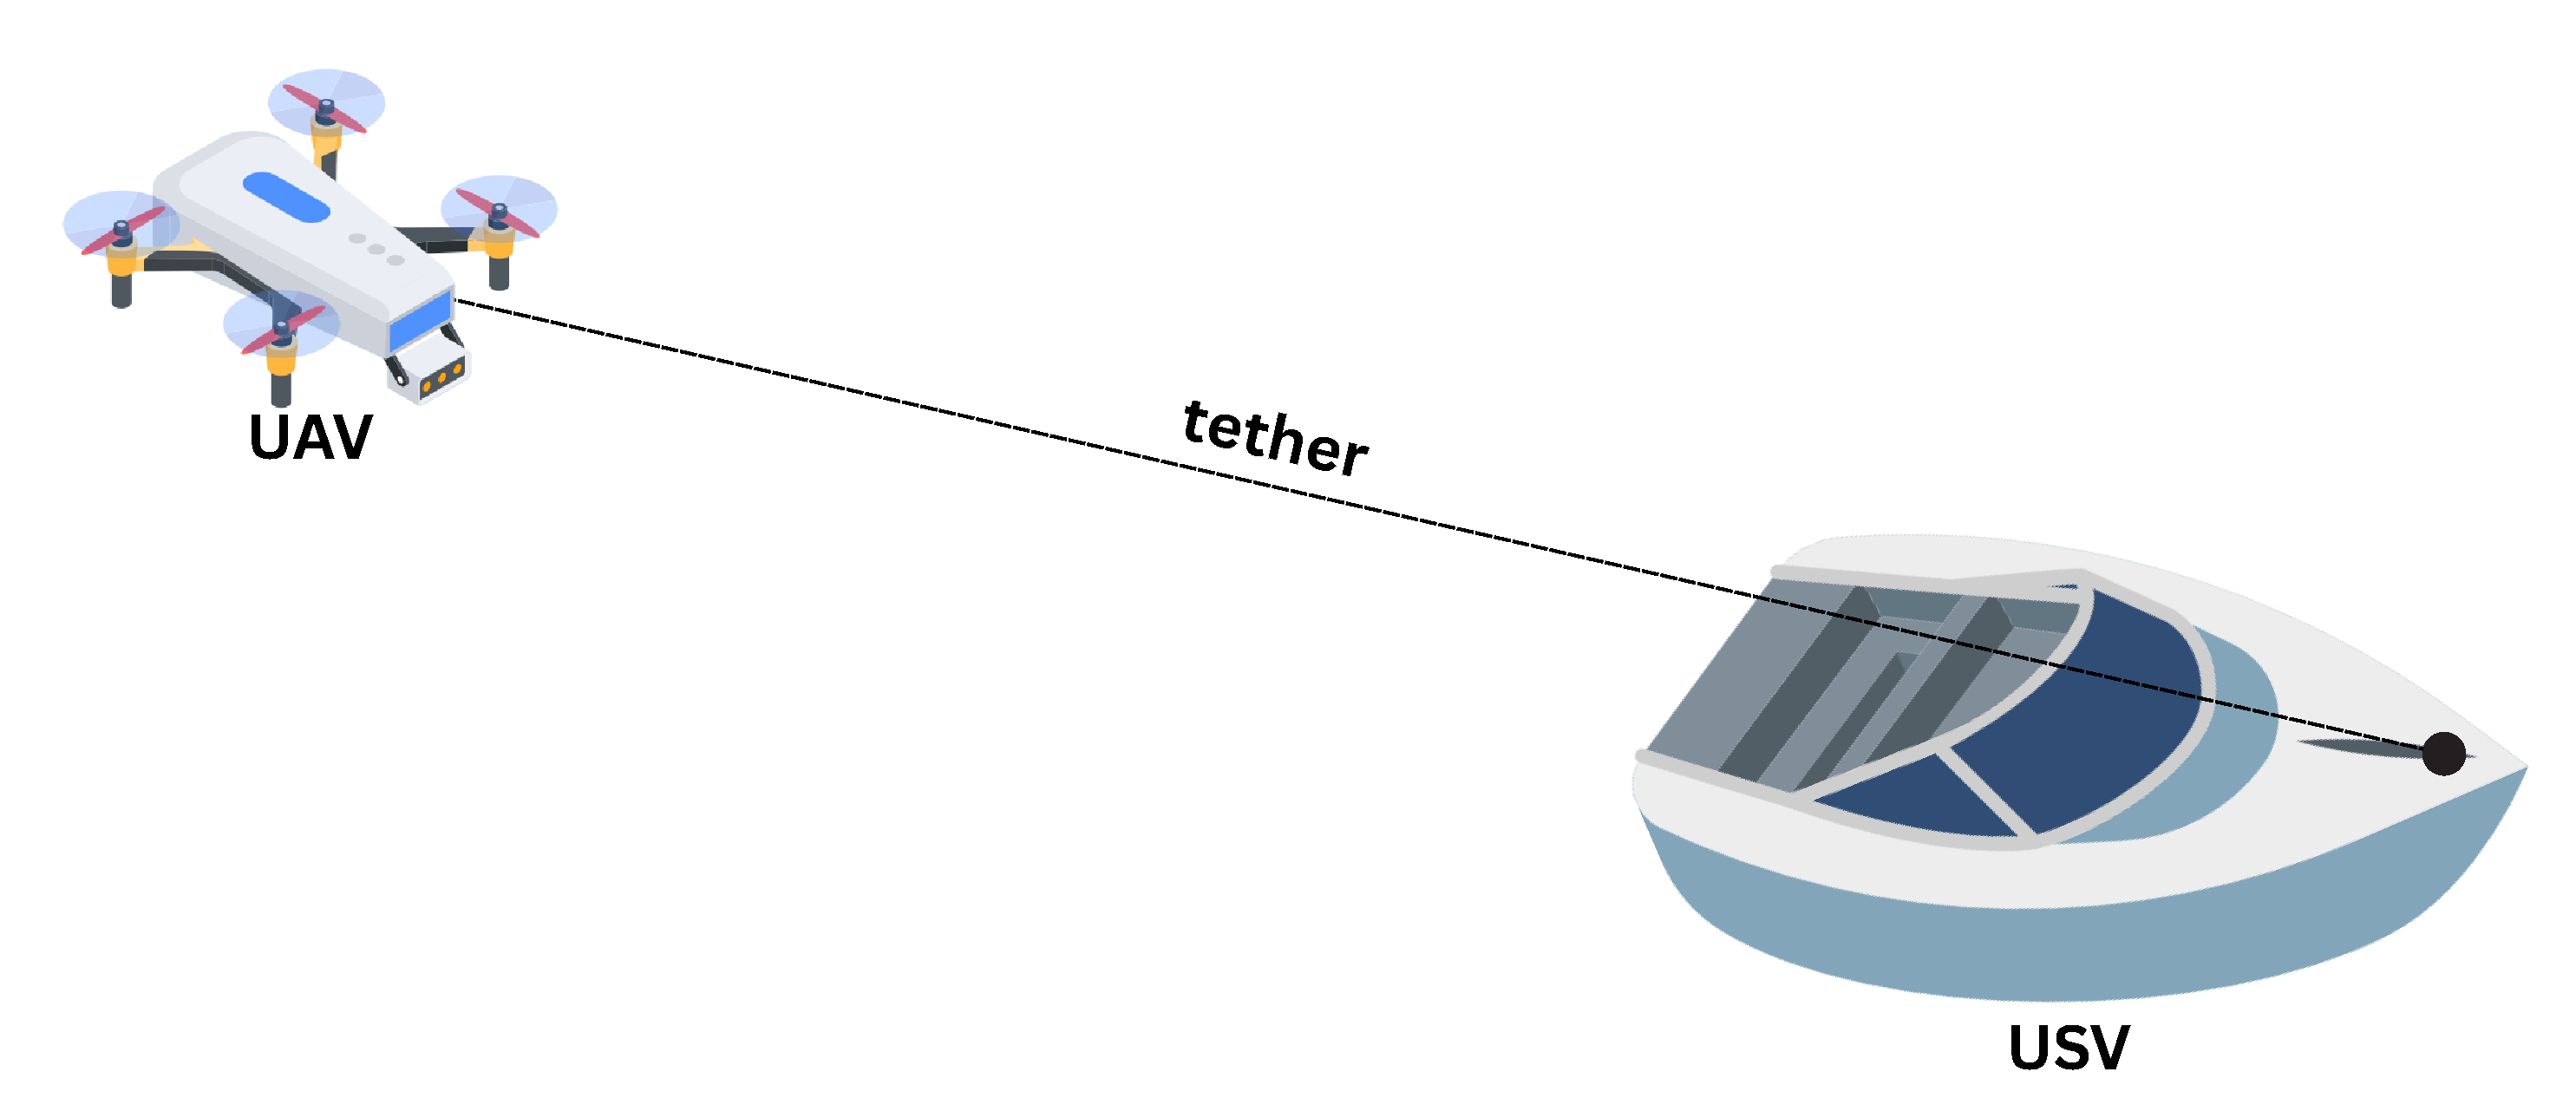
\includegraphics[width=0.6\linewidth]{Figures/introduction/system.pdf}
    \caption{Schematic of a tethered \gls{usv}--\gls{uav} system.}
    \label{fig:tether_scheme}
\end{figure}


% What problem are we solving?
The main challenge of this work is to design a control framework that enables two autonomous vehicles, connected by a tether, to operate as a single coordinated system. 
The controller must manage not only the motion of both vehicles but also account for the tether constraints and dynamics, ensuring safe operation and robustness to wind, waves, and obstacles.

The \gls{usv} and \gls{uav} operate under very different dynamics. 
The \gls{usv} moves slowly, dominated by hydrodynamic drag and inertia, while the \gls{uav} reacts quickly, with motion evolving on much shorter time scales. 
Coordinated control is challenging because the controller must handle these different response rates and actuation dynamics consistently.

The maritime environment adds further complexity. 
Wind, waves, and water motion constantly disturb both platforms, making robustness to disturbances essential. 
Nearby structures, vessels, or obstacles can restrict their movement and risk tether entanglement. 
Effective cooperation relies on continuous information exchange and synchronised decision-making between both agents.

Most existing tethered \gls{uav} systems focus on power delivery and communication, with operation often remaining manual or semi-autonomous. 
In research prototypes, the aerial and surface vehicles are usually decoupled, the tether is simplified or linearised, or the surface platform is treated as fixed. 
These assumptions make control design easier but reduce realism. 
Few cooperative control approaches explicitly model the tether while coordinating both agents under realistic maritime conditions.





%%%%%%%%%%%%%%%%%%%%%%%%%%%%%%%%%%%%%%%%%%%%%%%%%%%%%%%%%%%%%%%%%%%%%%%%
% \section{Work Objectives}
% \label{section:objectives}

% The objective of this work is to design and implement a cooperative control framework that enables a surface vessel and an aerial vehicle to operate together as a single system. The work begins with the analysis of suitable cooperation architectures for the \gls{usv}--\gls{uav} system, including the selection between centralised and distributed approaches. In parallel, different control strategies are studied to identify techniques that are appropriate for the system dynamics, constraints, and mission requirements.

% Once the cooperation architecture and control approach are selected, the focus shifts to modelling in support of implementation. Models of the \gls{usv}, the \gls{uav}, and the tether are developed with the explicit goal of enabling control implementation, capturing the dominant dynamics and couplings required for real-time operation.

% Based on these models, motion control algorithms are implemented to compute the individual actuation of each agent while ensuring cooperative behaviour. The controllers operate across multiple control modes, such as area patrol, target following, take off, and landing. A mission management logic is developed to allow the system to autonomously switch between modes in order to complete full missions.

% The controllers are tested in a simulation environment under controlled and repeatable conditions. The implementation is designed to support future extension to real-world experiments.

% System performance is evaluated using control-focused criteria. These include trajectory and waypoint tracking accuracy, area coverage during patrol tasks, control effort, robustness to external disturbances, and safe management of the tether while respecting physical and operational constraints. The ability of the system to autonomously transition between control modes and complete full missions is also assessed.

\section{Problem Statement}
\label{sec:problem_description}

This work addresses the problem of controlling a cooperative system composed of a \gls{usv} and a tethered \gls{uav} operating in a coordinated manner. The objective of such a system is to autonomously execute maritime missions by following predefined waypoints or continuous reference trajectories, while respecting the physical and operational constraints of both platforms and of the tether that connects them.

To achieve this objective, the control framework must be capable of handling different phases of operation and mission requirements. This includes the definition of multiple control modes that allow the system to perform manoeuvres such as take-off and landing, as well as different forms of coordinated motion during navigation.


%%%%%%%%%%%%%%%%%%%%%%%%%%%%%%%%%%%%%%%%%%%%%%%%%%%%%%%%%%%%%%%%%%%%%%%%
\section{System Overview}
\label{section:overview}

% System overview
Interaction with the system is defined at the mission level. The operator selects a mission, such as patrolling a given area, following a moving target, or visiting a set of waypoints that represent regions of interest. This mission information is received by a behaviour management layer, which selects the active control mode and handles mission logic, including switching between different relative configurations of the \gls{uav} with respect to the \gls{usv}, as well as executing specific manoeuvres such as take off and landing.

Based on the selected mission and active control mode, the system generates coordinated motion for both the \gls{usv} and the \gls{uav}. This process combines planning and control to compute trajectories and actuation commands that satisfy vehicle and tether constraints while pursuing the mission objectives. The \gls{uav} motion is designed to exploit its aerial perspective, providing sensing capabilities that complement those of the \gls{usv}.
The resulting control actions are applied directly to each vehicle, ensuring coordinated behaviour throughout the mission.

Figure~\ref{fig:placeholder} presents a high-level block diagram of the proposed system,

\begin{figure}[H]
    \centering
    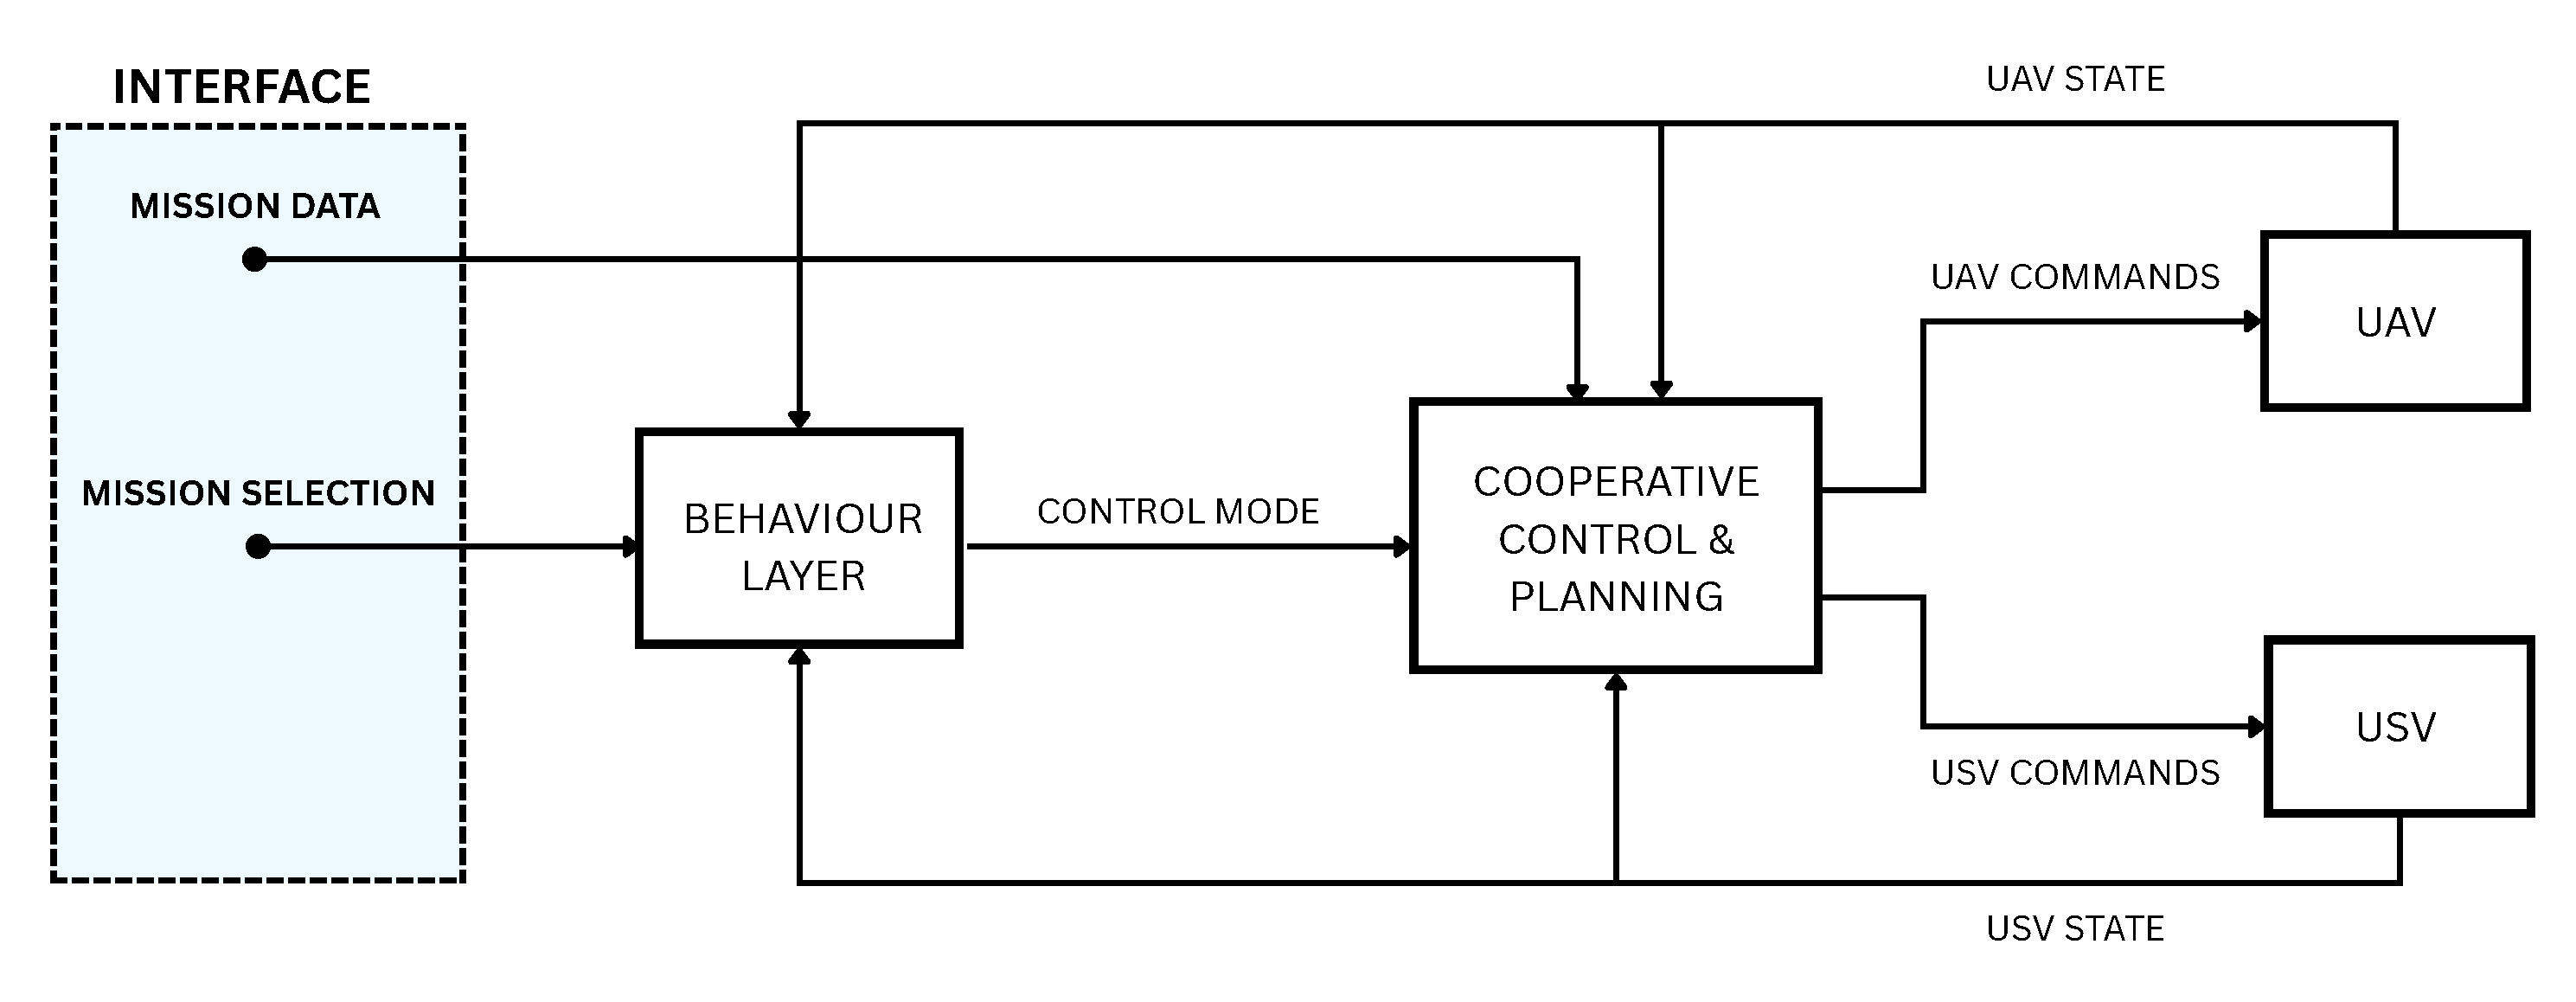
\includegraphics[width=0.9\linewidth]{Figures/introduction/block_diagram.pdf}
    \caption{Proposed System Block Diagram}
    \label{fig:placeholder}
\end{figure}

%%%%%%%%%%%%%%%%%%%%%%%%%%%%%%%%%%%%%%%%%%%%%%%%%%%%%%%%%%%%%%%%%%%%%%%%
\section{Expected Contributions}
\label{section:outline}


This thesis contributes to the design, implementation, and evaluation of cooperative control solutions for tethered \gls{uav}--\gls{usv} systems, to enable autonomous and persistent maritime missions. The main contributions of this work are summarised as follows:

\begin{itemize}
    \item A clear formulation of the cooperative control problem for a tethered \gls{uav} and an autonomous \gls{usv}, including the main constraints and couplings introduced by the tether and by the maritime operating environment.
    
    \item The development of control-oriented models of the \gls{uav}, the \gls{usv}, and the tether, capturing the dominant dynamics and interactions required for real-time control implementation.
    
    \item The design and implementation of a cooperative control framework capable of computing the individual actuation of both agents while ensuring coordinated behaviour across different mission phases.
    
    \item The definition and implementation of multiple control modes, such as area patrol, target following, take off, and landing.
    
    \item A simulation of the proposed cooperative control strategy under controlled and repeatable conditions.
    
    \item A systematic evaluation of system performance based on control-focused metrics, including tracking accuracy, control effort, robustness to external disturbances, and safe management of tether tension and geometry.
\end{itemize}
